\chapter{Evaluation}
\label{chap:analysis}

The Previous chapter introduced our approach on performance hot-spot detection of configurable software systems. Furthermore, it motivates the choice of the performance extraction tool by evaluating different extraction tools. In this chapter, we discuss the main question of this thesis: \emph{Can we identify performance hot-spots in configurable software systems?} In order to answer this question, we evaluate the applicability of our approach with a case study and answer the following research questions:


\begin{researchq}
	\item How can we define the configuration space of software systems?
	\label{rq:config_space}

	\item How strong is the impact of external influences on performance measurements?
	\label{rq:external_influence}
	
	\begin{researchq}
		\item Are the external influences workload sensitive?
		\label{rq:ext_inf_sensitivity}
		\item How does the \ac{GC} influence performance prediction of single methods?
		\todo{Tests}
	\end{researchq}

	\item Are performance hot-spots configuration or workload sensitive?
	\label{rq:sensitivity}

	\item Can we learn performance influence models on method level?
	\label{rq:perf_infl_model}

	\begin{researchq}
		\item How much information can we get by using pair-wise interactions instead of feature-wise??
		\label{rq:interactions}
		\item What influences the learning of performance-influence models?
		\label{rq:learning influence}
	\end{researchq}

\end{researchq}

% One top level RQ per chapter of results?
% 

This chapter is organized as follows. Section~\ref{test_env} defines the test environment we used to run our experiments. In section~\ref{case_studies} we present our subject systems. This includes a general description of each system, in order to motivate the choice to use these three for our chase study. We present in this section our method on how to extract the variability models of the subject systems to answer \ref{rq:config_space} and give an overview of the individual features that they implement. After that, we present the our results in section~\ref{results}. This includes our findings about the external measurement influence as well as the results of the performance-influence modelling process. Thereafter, section~\ref{discussion} evaluates the results by answering \ref{rq:sensitivity}, \ref{rq:perf_infl_model} and the corresponding sub-questions. The next section provides a detailed analysis of two topics of this thesis. First, we analyze the impact of external influences on our approach to answer \ref{rq:external_influence}. Especially, the influence of the \ac{GC} on performance prediction will be analyzed. The second topic presents the benefits of the provided visualisations by discussed some scenarios. Finally, section~\ref{validity} refers to assessing the reliability of the whole approach. 


\section{Measurement Setup}
\label{test_env}

All experiments were conducted on three dedicated computers, each with a Intel(R) Core(TM) i7-7700K CPU @ 4.20GHz, 32GB DDR4 RAM, and 500 GB SSD. Not only the hardware, but also the system software disposes of a homogeneous infrastructure. The \ac{OS} of the computers is Ubuntu 16.04.3 LTS 64 bit. There are the runtime systems for Python 3.5.2 and for Java OpenJDK Runtime Environment version 1.8.0\_171 installed. Except Python and Java, there is no additional software installed which could influence the measurements. 

As already mentioned in section \ref{perf_measure_system}, we configured each experiment execution to use one physical CPU core without overclocking. Before the measurements, the \emph{turbo\_boost.sh} script (the script is presented in the appendix~\ref{script_overclocking}) is executed. This script searches for all available CPU cores and disables or enables the turbo boost functionality of Intel CPUs with help of the \emph{wrmsr} tool. Each measurement, which refers to each execution of each single subject system with one configuration and one workload, is then executed with the command \emph{taskset 0x1 python3 profiling\_script\_random.py} which forces the Linux scheduler to keep the called process on the defined CPU. After this, other processes will be assigned to the remaining cores, because the core \emph{0x1} already has an increased workload because of our script.


%3 times:
%Intel(R) Core(TM) i7-7700K CPU @ 4.20GHz, 3512 MHz
%Nvidea GeForce GTX 1080 Ti
%32GiB System Memory:  32GB DDR4 2667 MHz
%OS name:         Linux
%OS architecture: amd64
%OS version:      4.13.0-39-generic
%Software:
%Java Version:    1.8.0\_161

%system settings:
%used one dedicated  cpu
%overclocking
%vm properties

\section{Subject Systems}
\label{subject_systems}

In the following, we present the subject systems we use in our case study. We choose three representative Java projects in order to analyze their performance behaviour. The subject systems are: \textit{Catena} password hashing framework, \textit{H2} SQL database, and \textit{Sunflow} rendering system for photo-realistic image synthesis. All three systems are \ac{OSS} projects written in Java. Each of them is a configurable software system with the possibility to customize their workload. 

To seek out the configuration space of the subject systems, we followed the guideline provided by \cite{Han:2016:ESP:2961111.2962602}. Because each software system can be implemented and documented in different ways, we had to study all artifacts that are publicly available to users including documentations (e.g., readme files, user manuals, online help pages), configuration files (e.g., default configuration examples, user manuals), and the source code itself. The ability to search the source code and test files, is another advantage of using \ac{OSS}. After identifying all configuration options, we combined by creating the corresponding feature models. This feature models can be used to calculate the whole configuration space and to sample a set of configurations for the experiments. Besides the identification of the configuration options, the possible workload of each system must be identified. Because each of these software systems is defined their possible workloads differently, we again had to search through all available material. 

%Eingrenzung auf Java software because, widespread, popular, often used, runs on billions of devices
%Decoding of Numerical features Is indicated through \_MIN\_MAX
%Configuration space calculation
%Because White-Box Testing explaination of individual features.

% 3 Java projects 
% 3 different kinds of projects to depict variety
% Configurable, Workload of projects to manage execution time and to validate results of projects with different workloads
% different configuration space 
% different ammount of configuration options
% 
% Definition of configuration space for subject systems\cite{Han:2016:ESP:2961111.2962602}:
% collection of information with studying all artifacts that are publicly available to users including documents (e.g. user manuals and online help pages), configuration files, and source code. -> anoter reason for open sourece projects because else there were only provided configurations available 

% proveded performance tests for the case studies
% Configuration space definition(\cite{Han:2016:ESP:2961111.2962602}): they also described the configuration space not only by parameter, but also with hidden configuration options and system-specific configurations
% they also described the configuration space not only by parameter, but also with hidden configuration options and system-specific configurations
% -> This thesis: system configuration options are restricted to one system to be able to limit the overall configuration options
% configuration parameter cause 78%-92% of configuration-related performance bugs
% for this thesis we do not investigate 8%-17% of system-level configuration bugs

In the following, we introduce each subject system. We define their configuration space through variability models, introduce the workloads we used, and explain each configuration option. 

\subsection{Catena}

%intro
Our first subject system, Catena, is a flexible and provable secure password hashing framework. As a finalist of the \textit{Password Hashing Competition}\footnote{Password Hashing Competition ran from 2013 to 2015 as an open competition to establish a standard in hashing passwords to be secure against attackers (\cite{phc2015}).}, Catena has convinced because of its internal graph-based structure, which brings a huge time-memory tradeoff. With different configuration options, users can tune Catena to consume more time and/or memory to hash passwords. This property prevents that hashes can be massively computed in parallel on clusters of graphics cards, which might be a possible scenario. 

% feature extraction
The Catena project provides us with nine versions of the documentation (provided by \cite{catena2014medsec}) as well as with the implementation itself (available on \url{https://github.com/medsec/catena-java}) which contains the implementation of Catena and some default variants. We derive the set of configuration options by searching the documentation files and by analyzing the source code. From this set of configuration options we created the feature model presented in Figure~\ref{fm_catena}.

\begin{figure}
  \centering
  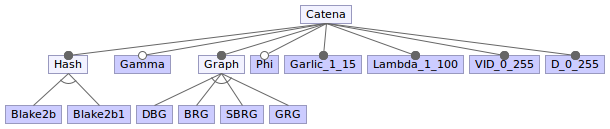
\includegraphics[width=0.8\textwidth]{images/Catena_Feature_model}
  \caption{Catena Feature Model.}
  \label{fm_catena}
\end{figure}

The Catena password hashing framework provides us with eight different features, three binary and 5 numerical. This results in a configuration space of \textbf{3,145,728,000} different possibilities (variants) to configure Catenas password hashing mode. In the following we give a short description of the features:

%Project size in Classes and Functions
%Project properties (SPL Model)
%Features explained
%Workload
%Num Dimensions: 3b 5n\todo{3+2b 4n}
%Whole configuration space: 3,145,728,000

\begin{description}[style=multiline,leftmargin=7em]
	\item [Hash] is a boolean parameter which defines the used hash function.
	\item [Gamma] is a boolean parameter (boolean) which adds a salt-dependent memory accesses layer to be resistant against attacks on dedicated hardware (e.g., ASICs\footnote{ASICs are hardware implementations of functions which are specialized to perform exactly a specific task.}), if enabled.
	\item [Phi] is a boolean parameter which adds functionality that adds additional security properties\footnote{If Phi is enabled, Catena is resistant against parallel computations of hashes. But Phi has the drawback that Catena becomes vulnerable against other attacks \cite{10.1007/978-3-319-29938-9_7}.}.
	\item [Graph] defines one out of four different graph structures, that defines the amount of necessary memory and time to compute the hash.
	\item [Garlic] defines time and memory requirements in a range from 1 to 15.
	\item [Lambda] defines the depth of the graph in a range from 1 to one 100.
	\item [VID] numerical value which decodes the unique version of Catena in a range from 0 to 255.
	\item [D] is an numerical parameter which is hashed together with other parameters to make up the tweak (increasing the additional computational effort for an adversary) in a range from 0 to two 255.
\end{description}

To execute Catena, we have to pick a configuration and we have to define a workload. A workload for Catena consists of three parameter: the password to be hashed, an user defined salt, and the output length of the hash. Table~\ref{wl_catena} presents the three workloads we used. The first workload consists of an empty password string, an empty salt string, and an output length of one. With this workload we tried to minimize the amount of computations Catena has to perform. The second workload is exactly the half in each parameter and the last workload is an example workload we have taken from the Catena test vectors repository\footnote{The Catena test vactore are available on \url{https://github.com/medsec/catena-test-vectors}.}.

\begin{table}
% Include Profiling Overhead and Accuracy to table

	\centering % Center table
    \begin{tabular}{*{9}{c}}
    	\toprule
        \# &Password & Salt & Output Length \\
        \midrule
        1 & '' & '' & 1 \\
        \midrule
        2 & '012345012345012345012345' & '6789ab6789ab' & 32 \\
        \midrule
        3 & \makecell{'012345012345012345012345'+ \\ '012345012345012345012345'} & \makecell{'6789ab6789ab'+ \\ '6789ab6789ab'} & 64 \\
        \bottomrule
    \end{tabular}
    \captionof{table}{Catena Workloads.}
    \label{wl_catena}
\end{table}


\subsection{H2}

% description
The next subject system we used is the H2 database engine. It is a pure Java SQL database with the aim to be one of the fastest \ac{OSS} databases. They performed performance benchmarks in comparison to other databases (e.g., HSQLDB, Derby, PostgreSQL, and MySQL) which yields that H2 is faster than the other databases, but consumes more memory\footnote{Performance benchmark results and descriptions of the used test cases are available on \url{http://h2database.com/html/performance.html}.}.

% Configuration space extraction
The H2 project provides a detailed online documentation\footnote{Documentation of parameters is available on \url{http://h2database.com/javadoc/org/h2/engine/DbSettings.html}.} for configuration options, usage scenarios, benchmark results, and other useful information. We extracted the set of configuration options from the documentation and created the feature model (shown in Figure~\ref{fm_h2}). In total we extracted fourteen binary options and two numerical options which result in a configuration space of 3,920,000,000 different variants. 

%Project description
%Project size in Classes and Functions
%Project properties (SPL Model)
%Features explained
%Workload
%Num dimensions: 14b 2n
%Whole configuration Space: 3,920,000,000

\begin{figure}
  \centering
  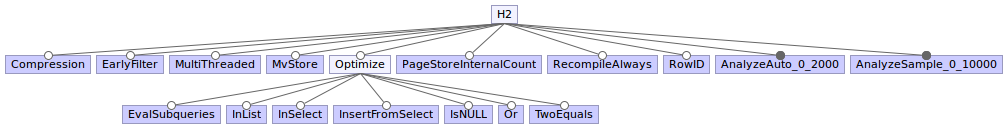
\includegraphics[width=\textwidth]{images/H2_Feature_model}
  \caption{H2 Feature Model.}
  \label{fm_h2}
\end{figure}


We excluded some options, because they does not influence the performance behaviour of the database (e.g., \textit{databaseToUpper} writes database names always in uppercase or \textit{defaultEscape} defines the default escape character) or produce exceptions during execution of the performance tests (e.g., changing the default value of \textit{maxQueryTimeout} causes some queries to not be executed). In the following we describe all configuration options that we extracted from the available options:

\begin{description}[style=multiline,leftmargin=11em]
	\item [Compression] compresses data when storing.
	\item [EarlyFilter] allows table implementations to apply filter conditions early on.
	\item [MultiThreaded] enables or disables multi threading.
	\item [MvStore] enables use of the MVStore storage engine.
	\item [OptimizeEvalSubqueries] optimizes subqueries that are not dependent on the outer query.
	\item [OptimizeInList] optimizes the \textit{IN(...)} and \textit{IN(SELECT ...)} operations.
	\item [OptimizeInSelect] optimizes the \textit{IN(SELECT ...)} operation.
	\item [OptimizeInsertFromSelect] enables insertion into tables from queries directly by passing temporary disc storage.
	\item [OptimizeIsNull] enables the use of indexing with \textit{IS NULL} checks.
	\item [OptimizeOr] optimizes the \textit{OR} operation.
	\item [OptimizeTwoEquals] enables the optimization of the equality check.
	\item [PageStoreInternalCount] enables updating the internal row counts.
	\item [RecompileAlways] enables that prepared statements always gets recompiled.
	\item [RowID] adds the preudo-column \textit{\_ROWID\_} to each table.
	\item [AnalyzeAuto] is a number which defines the necessary number of changes of rows in a table before the table gets analyzed.
	\item [AnalyzeSample] is a number which defines how many samples of a table gets analyzed.
\end{description}

% workload is the size of the database [10,000; 55,000; 100,000]
% performance extraction functionality are the tests of the benchnmark
We define the workload of H2 to be the available data in the database before the individual test are executed. We initialized the tables of the database we used in each test case with 10,000 rows for the first workload, 55,000 for the second workload, and 100,000 rows for the third workload. As the tasks the database has to perform, we make use of the benchmark which was used to conduct the performance comparison with the other database engines.

\subsection{Sunflow}

The last subject system we used in our case study is the rendering engine Sunflow. It is an \ac{OSS} project written in Java. Sunflow is build around a ray tracing core to create photo-realistic images with the help of many different features like camera motion blurring, lightmap generation, texture mapping, normal mapping, and other features. 

We wanted to analyze the performance of the process of rendering an image. Therefore, Sunflow already provides a benchmark which analyzes the resulting image (by time and by image quality) while modifying different parameters. We extracted all parameter that have changed (\textit{DiffuseDepth},\textit{ReflectionDepth}, and \textit{RefractionDepth}), to create the feature model of Sonflow. Furthermore, identified three more parameters (\textit{Threads},\textit{BucketSize}, and \textit{Samples}), which were hard-coded in the source code of the benchmark. These configuration option build up the feature model (shown in Figure~\ref{fm_sunflow}). Sunflow provides additional configuration options for different use cases. The GUI which comes with Sunflow can be modified by several options. Also the benchmark process can be adjusted, but we wanted to stick to the process of generating one image by using the standard scene (the cornell box with two tea pods and two glass balls).

\begin{figure}
  \centering
  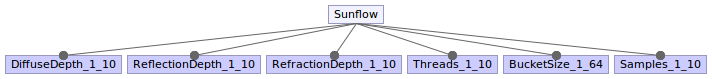
\includegraphics[width=\textwidth]{images/Sunflow_Feature_model}
  \caption{Sunflow Feature Model.}
  \label{fm_sunflow}
\end{figure}

In total we have a configuration space of 6,400,000 variants. In the following, we present a short description of all configuration options we used:

%Project description
%Project size in Classes and Functions
%Project properties (SPL Model)
%Features explained
%Workload
%Num dimensions: 6n
%Whole configuration space: 6,400,000

\begin{description}[style=multiline,leftmargin=11em]
	\item [DiffuseDepth] controls the maximum depth of diffuse light paths in the scene. 
	\item [ReflectionDepth] controls the maximum number of reflections a ray can do in the scene.
	\item [RefractionDepth] controls the maximum number of refractions a ray can do in the scene.
	\item [Threads] number of threads used for calculating the image in parallel.
	\item [BucketSize] defines the size of a moving window.
	\item [Samples] number of times the scene gets rendered.
\end{description}

As the different levels of workload we have take the resolution of the resulting image (64x64 pixel, 128x128 pixel, and 256x256 pixel). With these workloads we increased the workload by a quadruple. 

\rqparagraph{\ref{rq:config_space} \textit{How can we define the configuration space of software systems?}}
To define the configuration space of software systems we have to extract each configuration option that can be used to define the behaviour of the systems. A common way in black-box approaches is to search through documentations (online documentation or user manuals), readmes, and explore the interfaces the software provides. Because we use a white-box approach, we have also the possibility to extract options that are hidden while using black-box approaches. We used this chance to increase the amount of configuration options for our subject systems. But this comes with the drawback that the configuration space at least doubles itself with each option. However, with this approach, we can identify configuration options that might lead to an increased performance.



\section{Results}
\label{results}
% Present raw results and answer RQs
The following section presents the results of this thesis. We want to focus of the influences on our measurements in Section~\ref{ext_measurement_infl}. We also show which methods are sensitive for different configurations in Section~\ref{conf_sens} and which methods are sensitive for different workloads in Section~\ref{wl_sens}. Furthermore, we present the performance-influence models of each of our subject systems. Finally, we utilize our white-box approach by presenting the performance influence of the configuration options on each method in Section~\ref{perf_infl_models_m_lvl}.

\subsection{External Measurement Influence}
\label{ext_measurement_infl}

It is important to know the influence on measurement results when we run our experiments on real hardware. We restricted some sources of non-determinism to reduce their influence (hardware setup, installed software, and \ac{JVM} settings). By executing each workload with each configuration of each subject system (\textit{test case}) several times, we can detect differences in performance. We executed each test case seven times and determined the amount of variation of each test case. Figure~\ref{box_measure_infl_catena} shows the standard deviation of Catena of the three defined workloads (defined in Section~\ref{wl_catena}) of all sampled configurations. It can be seen that about half of the configurations are influenced only by 2.4\% or less. Furthermore, changing the workload does not have an influence on the variance of the measurement results. 

\begin{figure}
  \centering
  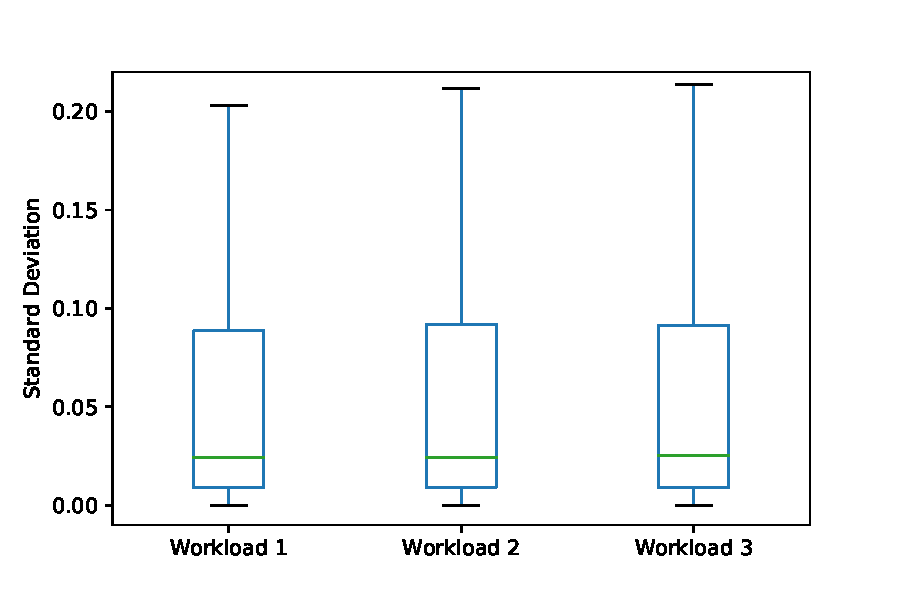
\includegraphics[width=0.6\textwidth]{images/catena_m_infl_wl_012}
  \caption{Measurement Influence of Catena with all Configurations (\#1000).}
  \label{box_measure_infl_catena}
\end{figure}

Figure~\ref{box_measure_infl_h2} shows, that there is a difference in the variance of the standard deviations with different workloads. The variance of the standard deviations is the biggest with the fist workload, the lowest with the second workload and increase again with the third workload. We expected, that with increasing runtime the influence decreases, because, for example, JIT compilation should have the highest influence at the start of the program. A possible reason for the higher variance of the measurements of the third workload might be the increasing amount of memory access. 

\begin{figure}
  \centering
  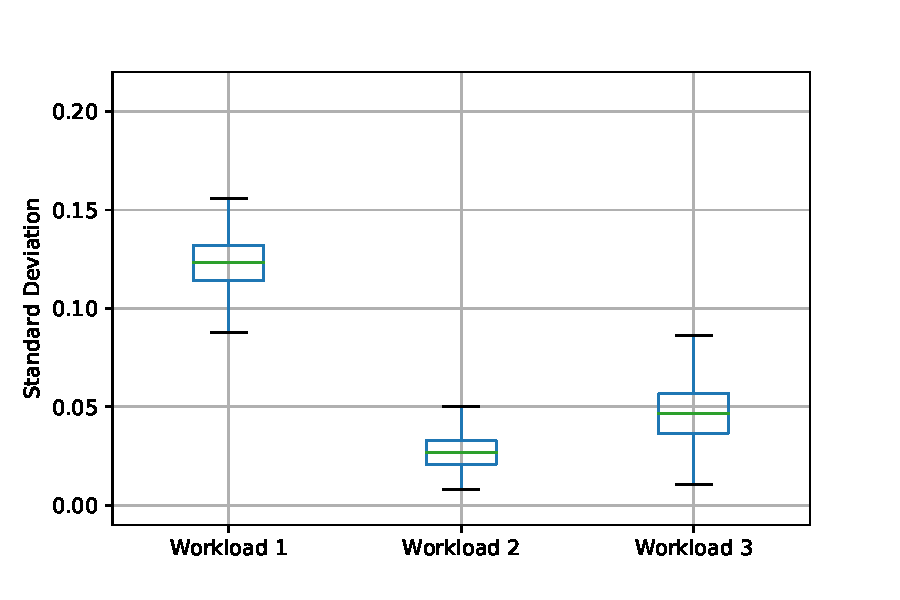
\includegraphics[width=0.6\textwidth]{images/h2_m_infl_wl_012}
  \caption{Measurement Influence of H2 with all Configurations (\#1000).}
  \label{box_measure_infl_h2}
\end{figure}

The variation in the measurement influence of Sunflow (see Figure~\ref{box_measure_infl_sunflow}) is as we expected it. The influence, as well as the variance in the influence decreases from the first workload to the third. In contract to the measurements of the workloads of H2, the influence of non-deterministic factors is less for all workloads.

\begin{figure}
  \centering
  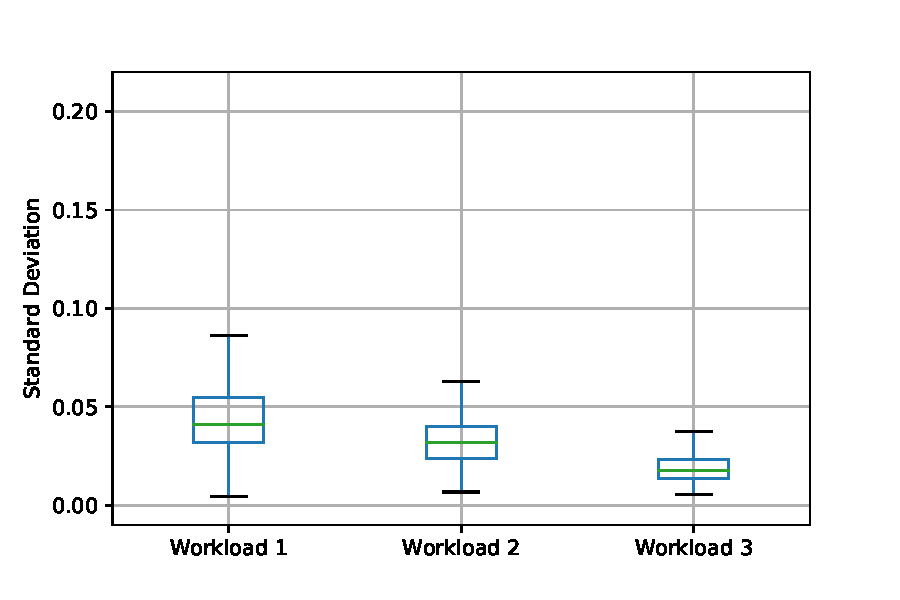
\includegraphics[width=0.6\textwidth]{images/sunflow_m_infl_wl_012}
  \caption{Measurement Influence of Sunflow with all Configurations (\#1000).}
  \label{box_measure_infl_sunflow}
\end{figure}

Because Catenas measurement variance remains the same for all workloads, we changed the parameter \textit{Garlic} from a maximum of 15 to 17 (only for this measurement influence test). Hereafter, the tests run for four times the time (increasing \textit{Garlic} by one doubles the runtime). But we can see in Figure~\ref{box_measure_infl_catena_x4} that the variance in the influence, as well as the amount of influence decreases. 

\begin{figure}
  \centering
  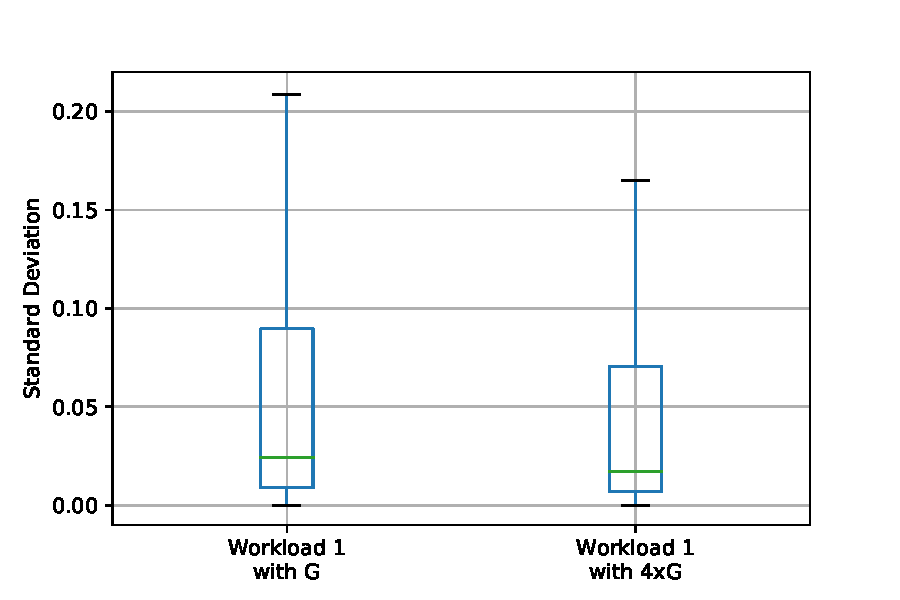
\includegraphics[width=0.6\textwidth]{images/catena_m_infl_wl_and_wlx4_0}
  \caption{Measurement Influence of Catena with all Configurations (\#820).}
  \label{box_measure_infl_catena_x4}
\end{figure}



\rqparagraph{\ref{rq:external_influence} \textit{How strong is the impact of external influences on performance measurements?}}
The mean external influence on our measurements is below five percent for all subject systems and workloads except for the H2 database engine. This high variance in the measurements of H2 under workload 1 may lead to inaccuracies in the remaining process. 

\rqparagraph{\ref{rq:ext_inf_sensitivity} \textit{Are the external influences workload sensitive?}}
But all systems tend to stabilize their performance with increasing runtime. Sunflow as well as Catena reached a mean variance of 2.5\% (Catena with increased \textit{Garlic} even 1.7\%)for their measurements with the third workload. 

%	\item How does the \ac{GC} influence performance prediction of single methods?


\subsection{Configuration Sensitivity}
\label{conf_sens}



\subsection{Workload sensitivity}
\label{wl_sens}

\subsection{Performance-influence Models}
\label{perf_infl_models}

\subsection{Performance-influence Models on Method Level}
\label{perf_infl_models_m_lvl}

% use quality metrics to describe
% Impact of configuration
% Impact of workload

\section{Discussion}
\label{discussion}

choice of workloads


\section{Detailed Analysis}
\label{delailed_analysis}

concentrate on Interesting parts
with help of developed tools we want to

\subsection{GC Analysis}
\label{gc_analysis}

impact of GC (Java specific stuff)
GC on/off
GC with different settings

\subsection{Eclipse Plugin}
\label{eclipse_plugin}

Eclipse plugin structure and functionality (maybe example usecase - what is better with this tool in comparison to others)
discussion of usage scenarios

\subsection{FlameGraphs}
\label{flame_graph}

Flame graph overview / idea, intention, usage scenario
discussion of usage scenarios

\section{Threads on Validity}
\label{validity}
How meaningful are our Results

\subsection{Internal Validity}

Which methodes and analyse metrics
Probably other profiler (more precise)


\subsection{External Validity}

Which environment and wich subject systems
